\documentclass[onecolumn,preprint,superscriptaddress,nofootinbib,notitlepage,10pt,linenumbers]{revtex4-1}
%
%=============================================================================
%\usepackage[margin=1.in]{geometry}
\usepackage{slashed}
\usepackage{graphicx}
\usepackage{amssymb}
\usepackage{mathtools}
\usepackage{bbold}
\usepackage{amssymb,latexsym}
\usepackage{amsmath,amsbsy,bbm}
\usepackage{multirow}
\usepackage[vcentermath]{youngtab}
\usepackage{nicefrac}
\usepackage[perpage]{footmisc}
\usepackage{wrapfig,lipsum,booktabs}
\usepackage{caption}
\usepackage{subcaption}
\usepackage{graphicx}
\usepackage{cjhebrew}

%\usepackage{physics}
\usepackage{floatrow}
\usepackage[dvipsnames]{xcolor} 
%\newfloatcommand{capbtabbox}{table}[][\FBwidth]
%=============================================================================
\newfloatcommand{capbtabbox}{table}[][0.45\textwidth]
%\DefineFNsymbols*{lamportnostar}[math]{\dagger\ddagger\S\P\|{\dagger\dagger}{\ddagger\ddagger}}
%\setfnsymbol{lamportnostar}
%\renewcommand\thefootnote{\fnsymbol{footnote}}
%=============================================================================
\usepackage{nicematrix}
\NiceMatrixOptions{
code-for-first-row = \color{blue} ,
code-for-last-row = \color{blue} ,
code-for-first-col = \color{blue} ,
code-for-last-col = \color{blue}
}

\newcommand{\es}{1\text{\scriptsize s}}
\newcommand{\zs}{2\text{\scriptsize s}}
\newcommand*{\mprime}{^{\prime}\mkern-1.2mu}
\newcommand{\largescale}{\ensuremath{\Lambda_\text{Hi}}}
\newcommand{\lc}{\ensuremath{\Lambda_c}}
\newcommand{\fm}{\ensuremath{\,\text{fm}^{-1}}}
\newcommand{\abb}{\mbox{\ensuremath{A\oplus 1}}}
\newcommand{\red}[1]{\textcolor{red}{#1}} 
\newcommand{\green}[1]{\textcolor{green}{#1}} 
\newcommand{\blue}[1]{\textcolor{blue}{#1}} 
\newcommand{\lec}{C^\Lambda}
\newcommand{\led}{D^\Lambda}
\newcommand{\ddrei}[1]{\delta_{\tiny \Lambda}^{(3)}\!\big(#1\big)}
\newcommand{\wrt}{\textit{w.r.t.}~}
\newcommand{\etc}{\textit{etc.}~}
\newcommand{\eg}{\textit{e.g.}~}
\newcommand{\ie}{\textit{i.e.}~}
\newcommand{\viz}{\textit{viz.}~}
\newcommand{\eftnopi}{\mbox{EFT$(\not \! \pi)$}}
\newcommand{\ve}[1]{\ensuremath{\boldsymbol{#1}}}
\newcommand{\rms}[1]{\ensuremath{\langle r(#1)\rangle}}
\newcommand{\ls}{\ve{L}\cdot\ve{S}}
\newcommand{\be}{\begin{equation}}
\newcommand{\ee}{\end{equation}}
\newcommand{\bra}{\big\langle}
\newcommand{\ket}{\big\rangle}
\newcommand{\hl}{\big\vert}
\newcommand{\vcl}[1]{\ensuremath{\bar{\boldsymbol{r}}_\text{\tiny #1}}}
\newcommand{\vsp}[1]{\ensuremath{\boldsymbol{r}}_\text{\tiny #1}}
\newcommand{\la}{\label}
\newcommand{\Pe}{\text{\cjRL{p|}}}
\newcommand{\figref}[1]{fig.~\ref{#1}}
\newcommand{\tabref}[1]{table~\ref{#1}}
\newcommand{\ccite}[1]{Ref.~\cite{#1}}
\newcommand{\dbra}[1] {\left\langle~#1~\right|}
\newcommand{\dket}[1] {\left|~#1~\right\rangle}
\newcommand{\bet}[1] {\left|#1\right|}
\newcommand{\overlap}[2] {\left\langle\,#1\,\left|\,#2\,\right.\right\rangle}
\newcommand{\me}[3] {\left\langle\,#1\,\left|\left.\,#2\,\right|\,#3\,\right.\right\rangle}
\newcommand{\redme}[3] {\left\langle\,#1\,\middle|\right|\,#2\,\left|\middle|\,#3\,\right\rangle}

\definecolor{blue}{HTML}{4169E1}
\definecolor{red}{HTML}{DC143C}
\definecolor{green}{HTML}{2E8B57}
\definecolor{mandarin}{HTML}{FF9933}

\newcommand{\MPV}[1]{\textcolor{purple}{#1}}
\newcommand{\LC}[1]{\textcolor{mandarin}{#1}}
\newcommand{\JK}[1]{\textcolor{green}{#1}}
\newcommand{\note}[1]{\textbf{\textcolor{gray}{#1}}}
%=============================================================================
\usepackage[normalem]{ulem}

\DefineFNsymbols*{lamportnostar}[math]{\dagger\ddagger\S\P\|{\dagger\dagger}{\ddagger\ddagger}}
\setfnsymbol{lamportnostar}
\renewcommand\thefootnote{\fnsymbol{footnote}}
\let\endtitlepage\relax

\begin{document}

\title{Universality of the multi-channel 4-body scattering system}
\author{Jean Luc Picard}
\email{jeanluc@1701.ncc}
\affiliation{Starfleet Academy, Fort Baker, San Francisco, Earth}
\date{\today}

\begin{abstract}
We investigate the scattering system of 4 equal-mass quantum particles at energies
where rearrangement channels are open. The interactions are renormalized to capture
the essence of the pertinent nuclear 2-neutron, 2-proton system. A full
treatment of the Coulomb interaction is included.

The quantity of most practical interest, namely the coupling between the deuteron-deuteron
and the ${}^3$H-proton/${}^3$He-neutron channels, is subjected to a sensitivity analysis
with respect to distorted, \ie, screened Coulomb repulsion between the two protons.
\end{abstract}

\maketitle

\paragraph{Few is more}

The fundamental question of interest is on the behaviour of 4
identical spin-$\nicefrac{1}{2}$ particles which can occupy 2
different isospin -- to stress the significance to systems other than
nuclei and mesons, we will use the more widely used notion of a flavour to discriminate
internal states of a fermion -- states.
We limit the investigation to the experimental most relevant 2-fragment
asymptotic configurations. These are defined by all partitions of the
$N=4$ particles into 2 clusters whose spectrum contains bound states.



Assuming zero-range, flavour\footnote{In nuclear physics the term 
isospin is more common to discriminate between internal states of a particle,
\eg, the neutron and proton, or the three charge states of a $\pi$ meson.} 
and spin-independent interactions 

the scattering process is parametrized via a 3-channel S-matrix:
\be
\la{eq.sm}
S_{ij}=\me{a\,L_a\,S_a}{\hat{S}^{J^\pi}}{b\,L_b\,S_b}=\eta_{ij}\,e^{2i\delta}
\;\;,\qquad
\ee

and the almost decoupled d-d channel is encoded in $\eta_{dd}\approx 1$. Although, the Coulomb repulsion between protons
provides a heuristic argument for this weak coupling, the comparison to the relatively strong coupling between the two 3-1
fragmentations seems to defy the argument as an equally strong force keeps the proton out of 3-helium.

%--
\begin{figure}[tb]
\centerline{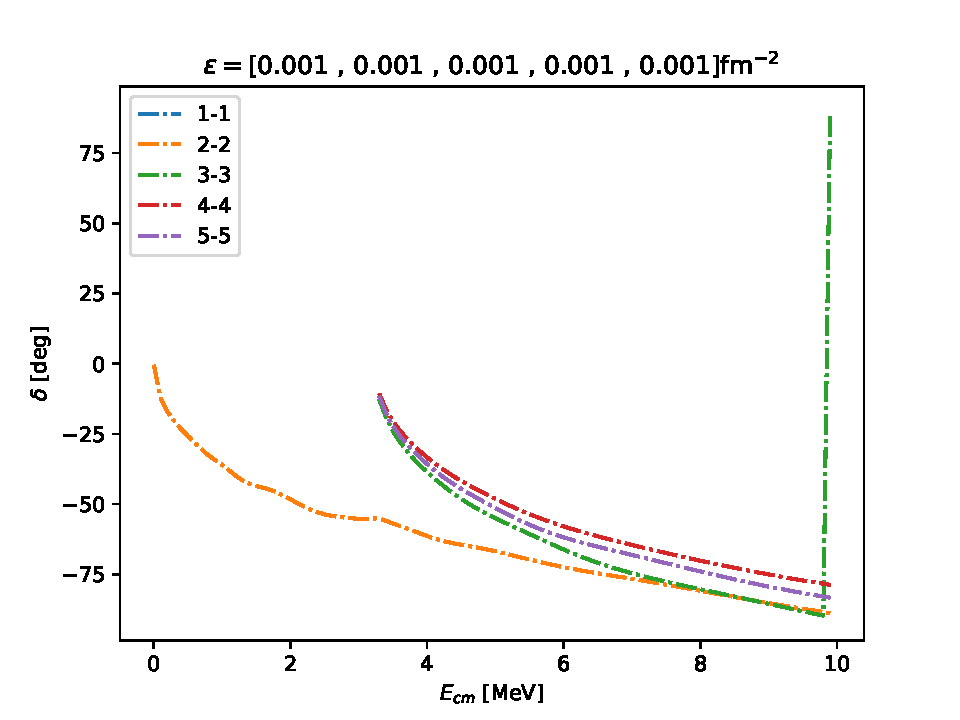
\includegraphics{/home/johannesk/kette_repo/limit_cycles/systems/4_lec_list_SU4/6.00/4_ph_0_6.0_lec_list_SU4.pdf}}
\caption{\label{fig.dd-phases} Energy dependence of phase shifts which parameterize the coupled channel
nnpp system in the ${}^1S_0$ $\alpha$ channel~\eqref{eq.sm}.
}
\end{figure}
%--

\paragraph{Spin-wave-function overlap}

\[
\begin{pNiceArray}{rrrr:rrr}[margin,first-row,first-col]
& \dket{\text{t-p}_1}  & \dket{\text{t-p}_6}&\dket{\text{he-n}_1}&\dket{\text{he-n}_6}&\dket{\text{d-d}}&\dket{\text{d}_q-\text{d}_q}&\dket{\text{nn-pp}}\\
\dbra{\text{t-p}_1}          & 6    &     & & & & & \\
\dbra{\text{t-p}_6}          &-6    & 6   & & & & & \\
\dbra{\text{he-n}_1}         &-2    &+2   & 0.66 & & & & \\
\dbra{\text{he-n}_6}         &-6    &+6   &+2 & 6 & & & \\
\hdottedline
\dbra{\text{d-d}}            &+8.5  &-8.5 &-2.8 &-8.5 & 12 &	 & \\
\dbra{\text{d}_q-\text{d}_q} &-4.9  &+4.9 &+1.6 &+4.9 &-6.9 & 4 & \\
\dbra{\text{nn-pp}}          &-4.9  &+4.9 &+1.6 &+4.9 &-6.9 &+4 & 4
\end{pNiceArray}
\]

\paragraph{Two-fragment approximation}

We expand a fragment state, $\overlap{\vcl{1}\ldots\vcl{A}}{\phi}$, which binds $A$ particles in a Gaussian basis
whose elements, $\overlap{\vcl{1}\ldots\vcl{A}}{m}$, are parametrized by $A$ width parameters $\alpha_{1\ldots A}^m$:
\[
\overlap{\vcl{1}\ldots\vcl{A}}{\phi}=
\sum_m\,c_m\cdot\overlap{\vcl{1}\ldots\vcl{A}}{m}=
\sum_m\,c_m\cdot e^{-\sum_i^A\alpha_i^m\vcl{i}}\quad.
\]

The basis is neither orthogonal nor normalized with a {\bf norm-matrix} element given by:

\begin{eqnarray}
\overlap{m}{n}&:=&
\underbrace{\int_{-\infty}^\infty\ldots\int_{-\infty}^\infty}_{6\times}
d^3(\vcl{1},\vcl{2})
e^{-\frac{1}{2}
\begin{bNiceArray}{c}
\vcl{1}\\\vcl{2}
\end{bNiceArray}^T
\cdot
\begin{bNiceArray}{cc}
2(\alpha_1^m+\alpha_3^m) & 2\alpha_3^m\\
2\alpha_3^m & 2(\alpha_2^m+\alpha_3^m)
\end{bNiceArray}
\cdot
\begin{bNiceArray}{c}
\vcl{1}\\\vcl{2}
\end{bNiceArray}
}
\cdot
e^{(m\leftrightarrow n)}
\nonumber\\
&=&\frac{\pi^3}{8\left[(\alpha_1^m+\alpha_1^n+\alpha_3^m+\alpha_3^n)(\alpha_2^m+\alpha_2^n+\alpha_3^m+\alpha_3^n)
-(\alpha_3^m+\alpha_3^n)^2\right]^{\nicefrac{3}{2}}}
\quad.
\end{eqnarray}

To obtain the expansion coefficients $c_i$ via a variational principle, we need to express the Hamilton operator
in the given basis.
The leading-order theory comprises a kinetic energy, a 2-, and a 3-body interaction term:

\[
\hat{H}\dket{\psi}=
\left[
(2m)^{-1}\sum^A_{i=1}\hat{p}_i^2
+\sum_{i<j}^A\delta^\lambda_{ij}
+\sum_{i<j<k}^A\delta^\lambda_{ij}\delta^\lambda_{ik}
\right]\dket{\psi}
\quad.
\]
In coordinate representation, we obtain the kinetic-energy matrix elements in the Gaussian basis:

\begin{align}
\me{m}{\sum_i\hat{p}_i^2}{n}
&=
\me{m}{\sum_i\hat{p}_i\,\hat{p}_i}{n}=
\sum_i\int d^3(\vsp{1\ldots A})\me{m}{\hat{p}_i}{\vsp{1\ldots A}}\me{\vsp{1\ldots A}}{\hat{p}_i}{n}\\
&\stackrel{\vsp{i}\to\vcl{i}}{=}
\end{align}

\bibliography{refs}

\end{document}